% 第 18 题正方体平面展开图＋直观图（两幅一体）：按固定源内容流矢量层精确值复刻（1 pt → 0.03515 cm，与全库同制）。
% 原点取展开图左上角 x=917.4062 pt、底缘 y（顶向下）=668.4500 pt（直观图 A/B 标签下缘）；y 向上。
% 源实测（figure-inventory §3）：
% 左幅（展开图）：十字六连方（竖条 1×4 叠横条 3×1 共用中格）；格边长 28.3359；
%   竖条轮廓 x 28.3360–56.6719、y 12.8355–126.3992；横条轮廓 x 0–85.0078、y 69.7273–98.0633；
%   竖条内部第 3 条格线 @ y 41.3914。8 个字母全部贴网格顶点排印（锚点见 figure-inventory §3.1.1）。
% 右幅（直观图）：8 顶点/12 棱（9 实 + 3 虚，虚线节距 2.98883，均自隐藏点 BBL 出发）；
%   前面 68.0117 × 64.1211（非严格斜二测，纵向压缩 5.72%，照源复刻）；深度偏移 (+24.0430, −24.0430)。
% 源内异常（照源复刻、已登记）：展开图与直观图 A–E 标注互为镜像（见试题文件存疑登记②）。
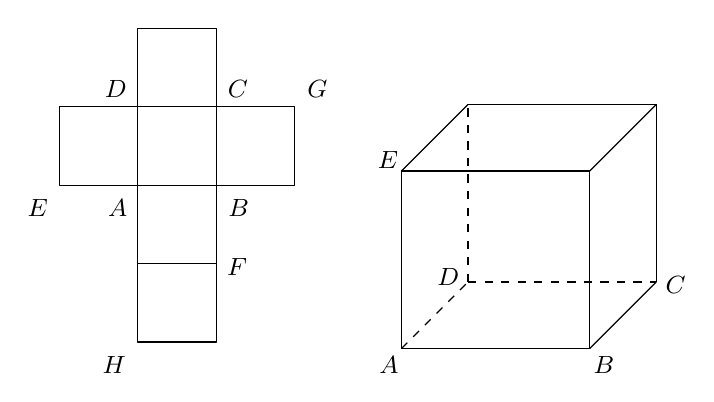
\begin{tikzpicture}[x=0.03515cm,y=0.03515cm,every node/.style={font=\small,inner sep=0pt},
  gl/.style={line width=0.398bp,line join=round}]
% ===== 左幅：平面展开图（十字六连方，格边长 28.3359）=====
\draw[gl] (28.3360,13.0555) rectangle (56.6719,126.3992);   % 竖条外轮廓（1×4）（修复 2026-10-11：下边 12.8355→13.0555＝668.45−655.3945，图自查揪出 0.22pt 传抄误差）
\draw[gl] (0,69.7273) rectangle (85.0078,98.0633);          % 横条外轮廓（3×1）
\draw[gl] (28.3360,41.3914)--(56.6719,41.3914);             % 竖条内部第 3 条格线（R3/R4 分界）
% ===== 左幅字母（照源字形盒中心定位；全部锚于格点）=====
\node at (20.3550,104.2750) {\(D\)};
\node at (64.4900,104.2750) {\(C\)};
\node at (93.2090,104.2750) {\(G\)};
\node at (-7.8340,61.3560) {\(E\)};
\node at (21.0560,61.3560) {\(A\)};
\node at (64.7210,61.3560) {\(B\)};
\node at (64.1150,40.2950) {\(F\)};
\node at (19.7770,4.6620) {\(H\)};
% ===== 右幅：正方体直观图（顶点照源实测）=====
% 实线 9 条
\draw[gl] (123.5430,10.7000)--(191.5547,10.7000);   % 前面下边 A–B
\draw[gl] (191.5547,10.7000)--(215.5977,34.7430);   % 右面下边
\draw[gl] (123.5430,74.8211)--(191.5547,74.8211);   % 前面上边
\draw[gl] (191.5547,74.8211)--(215.5977,98.8641);   % 右面上边
\draw[gl] (215.5977,98.8641)--(147.5860,98.8641);   % 顶面后边
\draw[gl] (147.5860,98.8641)--(123.5430,74.8211);   % 顶面左边
\draw[gl] (191.5547,74.8211)--(191.5547,10.7000);   % 前/右公共竖棱
\draw[gl] (215.5977,98.8641)--(215.5977,34.7430);   % 后面右边
\draw[gl] (123.5430,74.8211)--(123.5430,10.7000);   % 前面左边
% 虚线 3 条（均自隐藏点 BBL 出发；节距照源 2.98883）
\draw[gl,dash pattern=on 2.98883pt off 2.98883pt] (123.5430,10.7000)--(147.5860,34.7430);  % 底面左边（A→隐藏点）
\draw[gl,dash pattern=on 2.98883pt off 2.98883pt] (147.5860,34.7430)--(215.5977,34.7430);  % 底面后边
\draw[gl,dash pattern=on 2.98883pt off 2.98883pt] (147.5860,34.7430)--(147.5860,98.8641);  % 后面左边
% ===== 右幅字母（照源字形盒中心定位）=====
\node at (118.7040,78.6700) {\(E\)};
\node at (140.4790,36.6940) {\(D\)};
\node at (222.6230,33.6440) {\(C\)};
\node at (119.0060,4.6620) {\(A\)};
\node at (196.6420,4.6620) {\(B\)};
\end{tikzpicture}
